%%%%%%%%%%%%%%%%%%%%%%%%%%%%%%%%%%%%%%%%%
% Classicthesis Typographic Thesis
% LaTeX Template
% Version 1.3 (15/2/14)
%
% André Miede (http://www.miede.de)
%
%%%%%%%%%%%%%%%%%%%%%%%%%%%%%%%%%%%%%%%%%
\documentclass[
%		twoside,
		openright,titlepage,numbers=noenddot,headinclude,%1headlines,
                footinclude=true,cleardoublepage=empty,
                BCOR=5mm,paper=a4,fontsize=11pt, % Binding correction, paper type and font size
                ngerman,american, % Languages
                ]{scrreprt} 
\usepackage[utf8]{inputenc}
\usepackage{shadethm}
\usepackage[normalem]{ulem}
\usepackage[authoryear,round,colon]{natbib}
\usepackage{comment}
\usepackage{bibentry}
\usepackage{todo}
\usepackage[]{units}
\usepackage{lineno}

\input{support/classicthesis-config}

\begin{document}

\frenchspacing % Reduces space after periods to make text more compact
\raggedbottom % Makes all pages the height of the text on that page
\selectlanguage{american} % Select your default language - e.g. american or ngerman

%\renewcommand*{\bibname}{new name} % Uncomment to change the name of the bibliography
%\setbibpreamble{} % Uncomment to include a preamble to the bibliography - some text before the reference list starts

\pagenumbering{roman} % Roman page numbering prior to the start of the thesis content (i, ii, iii, etc)
\pagestyle{plain} % Suppress headers for the pre-content pages



%\newenvironment{chapter-structure}{\section*{Structure}\hrulefill\par\tiny}{\par\hrulefill\vspace{1cm}}


%----------------------------------------------------------------------------------------
%	PRE-CONTENT THESIS PAGES
%----------------------------------------------------------------------------------------
%Stuff for definitions using shadethm
\newshadetheorem{definitions}{Definition}[chapter]
\newenvironment{definition}[1][]{%
  \definecolor{shadethmcolor}{rgb}{.9,.9,.95}%
  \definecolor{shaderulecolor}{rgb}{0.0,0.0,0.4}%
  \setlength{\shadedtextwidth}{\textwidth}
%  \setlength{\shadeboxrule}{1.5pt}%
  \begin{definitions}[#1]\hspace*{2mm}%
  
}{\end{definitions}}

%%%My personal environment stuff.
\newenvironment{chapter-abstract}{\section*{Abstract}\hrulefill\par}{\par\hrulefill\vspace{0.0cm}}
\newenvironment{chapter-summary}{\section*{Summary}\hrulefill\par}{\par\hrulefill\vspace{0.0cm}}

%Page number per chapter (starting with 0?)
\numberwithin{page}{chapter}
\renewcommand*{\cleardoublepage}{} %Remove empty pages
%\linenumbers

%%*******************************************************
% Titlepage
%*******************************************************
\begin{titlepage}
    % if you want the titlepage to be centered, uncomment and fine-tune the line below (KOMA classes environment)
    \begin{addmargin}[-1cm]{-3cm}
    \begin{center}
        \large  

        \hfill

        \vfill

        \begingroup
            \color{Maroon}\spacedallcaps{\myTitle} \\ \bigskip
        \endgroup

<<<<<<< HEAD
				\vspace{0.7cm}	
				vorgelegt von
				
				\vspace{0.7cm}	
				MSc. Dennis Guse
				
				geb. 24. Oktober 1984 in Berlin, Deutschland

				\vspace{1.7cm}
				an der Fakultät IV - Elektrotechnik und Informatik
				
				der Technischen Universität Berlin
				
				zur Erlangung des akademischen Grades

				\vspace{0.7cm}
=======
				vorgelegt von
				
				\vspace{0.5cm}	
				MSc. Dennis Guse
				
				geb. 24. Oktober 1984 in Berlin, Deutschland
				\vspace{1.5cm}				
				
				an der Fakultät IV - Elektrotechnik und Informatik
				
				der Technischen Universität Berlin
				
				zur Erlangung des akademischen Grades

				\vspace{0.5cm}
>>>>>>> ed74f9a2eddc220016fbcde7d2d2bc378959789c
				Doktor der Naturwissenschaften
				
				-- Dr. rer. nat. --

%				\vspace{0.5cm}
%				genehmigte Dissertation
<<<<<<< HEAD
				\vspace{2.2cm}
				
				\centering
				\large
				\begin{tabular}{ll}
				\multicolumn{2}{c}{Promotionsausschuss} \\
=======
				\vspace{1.5cm}
				
				\begin{table}[h!]
				\centering
				\begin{tabular}{ll}
				Promotionsausschuss: \\
>>>>>>> ed74f9a2eddc220016fbcde7d2d2bc378959789c
				\hline				
				(Vorsitzender) & tbd \\
				(Gutachter)	& Prof. Dr-Ing. Sebastian Möller \\
				(Gutachter)	& Prof. Dr. Judith Redi \\
				(Gutachter)	& Prof. Dr. Ulrich Reiter \\
				\end{tabular}
<<<<<<< HEAD
				
				\vspace{1.7cm}				
=======
				\end{table}
				
				\vspace{1cm}				
>>>>>>> ed74f9a2eddc220016fbcde7d2d2bc378959789c
				Tag der wissenschaftlichen Aussprache: tbd.

				\vspace{1cm}				
				Berlin, April 2016
%        \spacedlowsmallcaps{\myName}
%
%        \vfill
%
%        \mySubtitle \\ \medskip   
%        \myDegree \\
%        \myDepartment \\                            
%        \myFaculty \\
%        \myUni \\ \bigskip
%
%        \myTime\ -- \myVersion

        \vfill                      

    \end{center}  
  \end{addmargin}       
\end{titlepage}    % Main title page
%\thispagestyle{empty}

\hfill

\vfill

\noindent{}Dennis Guse: \textit{Multi-episodic Perceived Quality of Telecommunication Services}, %\myDegree, 
\textcopyright{} September 2016

%\bigskip
%
%\noindent\spacedlowsmallcaps{Supervisors}: \\
%\myProf \\
%\myOtherProf \\ 
%\mySupervisor
%
%\medskip
%
%\noindent\spacedlowsmallcaps{Location}: \\
%\myLocation
%
%\medskip
%
%\noindent\spacedlowsmallcaps{Time Frame}: \\
%\myTime
 % Back of the title page
%\cleardoublepage% Dedication

\thispagestyle{empty}
\refstepcounter{dummy}

\pdfbookmark[1]{Dedication}{Dedication} % Bookmark name visible in a PDF viewer

\vspace*{3cm}

\begin{center}
The remembering self is sometimes simply wrong. \\ \medskip
--- (Kahneman and Riss, 2005, p. 286)
\end{center}

\medskip

\begin{center}
Experiences are fleeting [whereas] memories are what we get to from our experiences. \\ \medskip

--- Mrion-Shatz et al. 2009 after Kahneman & Riis 2005, p. 286 (Not present here!)
\end{center}
 % Dedication page
%\cleardoublepage\include{support/FrontBackMatter/Foreword} % Uncomment and create a Foreword.tex to include a foreword
%\cleardoublepage%*******************************************************
% Abstract
%*******************************************************
%\renewcommand{\abstractname}{Abstract}
\pdfbookmark[1]{Abstract}{Abstract}
%\begingroup
%\let\clearpage\relax
%\let\cleardoublepage\relax
%\let\cleardoublepage\relax

\chapter*{Abstract}
Telecommunication services have to cope with degradations resulting from the transmission of data.
A telecommunication service might thus not be able to to provide the same performance for a user, if it is used repeatedly by this user.
If perceived, this variation in perceived quality might affect the user's satisfaction, attitude, behavior, and also future-use intention towards this telecommunication service.

In this thesis, the integration process towards the perceived quality over multiple, distinct interactions with one telecommunication service is investigated.
The integration process of the so-called multi-episodic perceived quality is investigated here for two time spans.
As a baseline repeated use in one multi-episodic session is investigated. %of up to \unit[45]{min}
This is complemented by investigating the integration process considering usage over several days.
This investigating was conducted by performing several empirical experiments under controlled laboratory settings and also under field situations.
These experiments are based upon the \acs{MOS}, \ie, let the perceived quality of (almost) identical stimulus/condition be assessed by multiple observers, to derive the judgment of an \emph{average observer}.
The impact of individual behavior is limited here by applying the defined-use method, \ie, defining the task, content, and also time for each episode as well as the performance level.
Besides verifying feasibility, the results of the experiments show that the integration the integration process resembles an averaging process with a higher impact of more recent episodes.
It could be observed that the found effects do not seem to depend on the duration of the experiments, \ie, one session versus multiple days.

%\vfill

\begin{otherlanguage}{ngerman}
\pdfbookmark[1]{Zusammenfassung}{Zusammenfassung}
\chapter*{Zusammenfassung}


\end{otherlanguage}
%\endgroup			
%\vfill
%\cleardoublepage\include{support/FrontBackMatter/Publication} % Publications from the thesis page
%TODO Add here a list with my own publications here; must descripe what I did for all work that has shared authorship.

%\cleardoublepage%*******************************************************
% Acknowledgments
%*******************************************************
\pdfbookmark[1]{Acknowledgments}{acknowledgments}

\bigskip

\begingroup
\let\clearpage\relax
\let\cleardoublepage\relax
\chapter*{Acknowledgments}
During my time working on my dissertation, I had the pleasure to meet, work, and getting to know a large number of awesome persons.

I would like to thank my supervisor Prof.~Dr\=/Ing.~Sebastian Möller for providing me the opportunity to pursue my doctoral degree.
Also, I would like to thank Prof.~Dr.~Judith Redi and Prof.~Dr.\=/Ing.~Ulrich Reiter for serving on my doctoral committee.
Also, I am grateful that I had the opportunity to work closely with Dr.~Benjamin Weiss, who provided important feedback, near-endless discussions, and his steady support.
The same holds for Prof.~Dr\=/Ing.~Alexander Raake.

My deepest thanks goes to my colleagues Anna Wunderlich and Frank Haase.
Without their impressive work, their clever ideas, and their precise preparation, the conducted experiments and thus this dissertation would have been impossible.
It felt like pure luxury working with them.
Thanks also to Henrique~R.~Orefice for the opportunity to build an awesome software project.

I would also thank my colleagues and friends Friedemann Köster, Falk Schiffner, Steffen Zander, Janto Skowronek, Dr.~Hagen Wierstorff, Dr.\=/Ing.~Sebastian Arndt, Johannes Rummel, Dr.~Oliver Hohlfeld, and Prof.~Dr.\=/Ing.~Jens Ahrens for introducing me to interesting topics, helped working on fancy research projects, and, most important, cheering me up.
Especially, the near-infinite number of table soccer games and the impressive niveau have been very important to me.

Last but not least, I am grateful to my girlfriend Regine Hähnel.
Without her energetic, continuous support, I would not finished my dissertation
I am so glad, she endured all the stressful times and helped enthusiastically.

\bigskip
It was pleasure to meet you all and being part of my life.

\bigskip
Thanks.

\endgroup

\pagestyle{scrheadings} % Show chapter titles as headings
\cleardoublepage%*******************************************************
% Table of Contents
%*******************************************************
%\phantomsection
\refstepcounter{dummy}
\pdfbookmark[1]{\contentsname}{tableofcontents}
\setcounter{tocdepth}{2} % <-- 2 includes up to subsections in the ToC
\setcounter{secnumdepth}{3} % <-- 3 numbers up to subsubsections
\manualmark
\markboth{\spacedlowsmallcaps{\contentsname}}{\spacedlowsmallcaps{\contentsname}}
\tableofcontents 
\automark[section]{chapter}
\renewcommand{\chaptermark}[1]{\markboth{\spacedlowsmallcaps{#1}}{\spacedlowsmallcaps{#1}}}
\renewcommand{\sectionmark}[1]{\markright{\thesection\enspace\spacedlowsmallcaps{#1}}}
%*******************************************************
% List of Figures and of the Tables
%*******************************************************
\clearpage

\begingroup 
    \let\clearpage\relax
    \let\cleardoublepage\relax
    \let\cleardoublepage\relax
    %*******************************************************
    % List of Figures
    %*******************************************************    
    %\phantomsection 
    \refstepcounter{dummy}
    %\addcontentsline{toc}{chapter}{\listfigurename}
    \pdfbookmark[1]{\listfigurename}{lof}
    \listoffigures

		\newpage

    %*******************************************************
    % List of Tables
    %*******************************************************
    %\phantomsection 
    \refstepcounter{dummy}
    %\addcontentsline{toc}{chapter}{\listtablename}
    \pdfbookmark[1]{\listtablename}{lot}
    \listoftables
    
	  \newpage
    
    %*******************************************************
    % List of Listings
    %*******************************************************      
      %\phantomsection 
%    \refstepcounter{dummy}
%    %\addcontentsline{toc}{chapter}{\lstlistlistingname}
%    \pdfbookmark[1]{\lstlistlistingname}{lol}
%    \lstlistoflistings 
%
%    \vspace{8ex}
       
    %*******************************************************
    % Acronyms
    %*******************************************************
    %\phantomsection 
    \refstepcounter{dummy}
    \pdfbookmark[1]{Acronyms}{acronyms}
    \markboth{\spacedlowsmallcaps{Acronyms}}{\spacedlowsmallcaps{Acronyms}}

\chapter*{Acronyms}
\begin{acronym}[POLQA]
\acro{AAC}{Advanced Audio Coding}
\acro{ACR}{Absolute Category Rating}

\acro{AoD}{Audio on Demand}

\acro{CCR}{Continuous Category Rating}
\acro{ETSI}{European Telecommunications Standards Institute}

\acro{FEC}{Forward Error Encoding}
\acro{FPS}{Frames per Second}


%\acro{GSM}{Global System for Mobile Communications}
\acro{H.264}{MPEG-4 Part 10, Advanced Video Coding}
\acro{HP}{High Performance}

\acro{HTML}{Hypertext Markup Language}
\acro{HTTP}{Hypertext Transfer Protocol}

%\acro{CT}{Conversation Test}

%\acro{NPS}{Net Promoter Score}
\acro{IP}{Internet Protocol}
\acro{ITU}{Internation Telecommunications Union}

\acro{LP}{Low Performance}

\acro{MOS}{Mean Opinion Score}
\acro{MP}{Medium Performance}

\acro{MP3}{MPEG-1 Audio Layer III}

\acro{QoE}{Quality of Experience}
\acro{QoS}{Quality of Service}
\acro{QP}{Quantification Parameter}

\acro{PLC}{Packet-loss Concealment}
\acro{POLQA}{Perceptual Objective Listening Quality Assessment}
\acro{RMSD}{Root Mean Square Deviation}

\acro{RTP}{Real-Time Transport Protocol}

\acro{SCS}{Short Conversation Scenario} %USE another abbreviation
\acro{SIP}{Session Initiation Protocol}
\acro{SSCQE}{Single Stimulus Continuous Quality Evaluation}
\acro{STUN}{Session Traversal Utilities for NAT}

\acro{VoD}{Video on Demand}
\acro{VoIP}{Voice-over-IP}

\acro{USB}{Universal Serial Bus}
\acro{UX}{User Experience}
\end{acronym}               
\endgroup

\cleardoublepage

%----------------------------------------------------------------------------------------
%	THESIS CONTENT - CHAPTERS
%----------------------------------------------------------------------------------------
\pagenumbering{arabic}\setcounter{page}{1}
%\part{Introduction and State of the Art}\cleardoublepage

\chapter{Introduction}\label{chap:01}
\begin{chapter-abstract}
Here I give an overview on my thesis.
This includes general topic and field of research (perceptual quality judgment that relies on memorization and then recall).
I state why this topic is relevant and what practical implications occur.
I give a brief overview on "service basics": to service, satisfaction, acceptance, money stuff.
At the end I will state the research questions and my approach towards answering this question.
I will give hints on the results a reader can expect.
\end{chapter-abstract}

%\section{Basic definitions}
%\begin{itemize}
%\item What is \emph{to service}? [Whitepaper] [http://www.merriam-webster.com/dictionary/service] 
%\item What is a service, application, system?
%\item Telecommunication services + Service Provider %https://www.law.cornell.edu/uscode/text/47/153#50
%\end{itemize}
%\paragraph*{Service provider's goal}
%Make customer happy for as little money as possible for infrastructure: 
%\begin{itemize}
%\item cost-efficiency: trade-off
%\item risk reduction
%\item Service usage
%\item repeated usage / churn
%\end{itemize}
%\section{Aspects}
%\begin{itemize}
%\item QoE as hygienic factor [Moeller, Wechsung]  
%\item Money: NPS, Churn, Acceptability, Willingness-to-paying
%\item Retainability (sMOS)
%\item Adaptive services: service that adjust performance to current conditions (best + economic feasible)
%\end{itemize}

A \emph{service provider} provides a \emph{service}\footnote{Please note that the term \emph{service} in this work does not refer to a technical system executed on a server.} that provides a defined "service" to potential users.
In difference to "product creating industries" a service cannot be pre-manufactured, but is rather created on request when needed by a then user., \ie to serve somebody.
%TODO: Performance cannot be determined beforehand! Trust; Service usage lifecycle? Customer Expectations and providers promise

Before actually deciding to use a service, a potential user must have a need that can be fulfilled by using a service. %proposes to fulfill
If multiple service provider that provide a similar service, a potential user must chose which service to use for fulfillment of his need.
When satisfied with the outcome of using the service a user might interact with the service later on again, whereas a non-satisfying outcome will likely result in not using the same service again and rather use a different one.
In fact, using the same service again, saves time and resource, because the service discovery, evaluation and selection is not conducted.

However, the performance of a service cannot be constant as the service is created on-demand.
The performance of a service might be varying from usage instance to usage instance.
From a user's perspective this might be sufficient, but if the performance some usage instances does meet the expectations / desired performance then a dissatisfaction might occur.
This force the user to abandon the service provider and chose a different one.

This is, in fact, holds for both \emph{physical services} in which a service is provided to user in a physical location often by a person, but also for \emph{telecommunication services}\footnote{Definition as bit pipe as of https://en.wikipedia.org/wiki/Telecommunicationsservice follow definition of US Communications Act of 1934} like speech telephony or Internet access.
In fact, in telecommunication service are different from classical services as those provide communication between one or more parties, which can be a computer or a person.

%Scope
In this work, I present my work on the \emph{perceived quality impression} occurring by a human user of telecommunication services.
This work extends prior work by investigating the impact of varying service/system performance on the perceived quality, when the same system(s) are used repeatedly.
This is, in fact, a common case for telecommunication service.
For example a customer of a mobile  provider will use the provided service(s) usually repeatedly, because his telephone number is bound to the service provider and, although it can be transfered to a different provider, this process takes time and effort.
Furthermore, a customer might be bound for a certain extend to a service provider contract duration.
Although contract duration might bind customers to a provider, low performance and thus a low perceived quality affects the future use behavior and increases the churn rate for the end of contract.
In addition, satisfaction and also dissatisfaction of a customers can spread to other customers and potential customers and thus have severe impact on the business performance of a service provider.

In this work I focus on the development of perceived quality over several distinct interactions with a telecommunication service and how a retrospective assessment of the perceived quality of this service is affected by varying service performance.
%TODO What is performance and what is perceived quality
The actual impact on customer satisfaction and thus business performance of performance variation is not in the scope of this thesis.

Two research questions are addressed in this thesis:
\begin{itemize}
\item How does perceptual quality evolve over multiple distinct interactions with the one system/service for one user?
\item How does perceptual quality evolve over multiple distinct interactions with a multiple services offered by the same service provider for one user?
\end{itemize}

Here distinct interaction refers to one usage instance by a user with a service to fulfill a certain need of the user or solve a certain task.
Such an instance is denoted as a \emph{usage episode}.
Each usage episode has a perceived quality, which can be assessed momentary while in the usage episode and also in retrospective after the usage episode is finished.
In this thesis I investigate how a multi-episodic perceived quality evolves over several distinct usage episode with the same service.

\begin{figure}
	\centering
	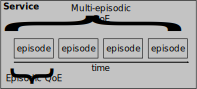
\includegraphics[width=1\columnwidth]{fig/multi-episodic}
	\caption{Repeated usage episodes with one service and their episodic QoE form a multi-episodic QoE in the user.}
	\label{img:chap01:multi-episodic}
\end{figure}

This thesis has two goals:
\paragraph*{Goal 1}
First, I will investigate what affects a retrospective multi-episodic quality judgment.
The major focus here is to understand which usage episode are of special importance for a multi-episodic quality judgment and what temporal effects occur.

\paragraph*{Goal 2}
Second, I will investigate how multi-episodic quality can be predicted based upon episodic quality judgments and investigate components for model.

\section{Structure}
This thesis is divided into two parts.
In \emph{Part I} I will introduce concepts and fundamentals that form the basis for my approach towards multi-episodic quality.
In Chapter~\ref{chap:02} an introduction on \ac{QoE} is given.
This includes prior work on psychophysics, perception and the quality formation process.
At the end of this chapter the relationship to higher level concepts like satisfaction and service quality is discussed.
In Chapter~\ref{chap:03} I present relevant concepts that affect recall and thus retrospective judgments of an \emph{general experience}.
Here, I will discuss how memory affects those retrospective judgments and those (temporal) effects are presented.
Based upon Chapter~\ref{chap:02} and Chapter~\ref{chap:03} I will present the state-of-the-art on performance fluctuations on QoE in one usage episode in Chapter~\ref{chap:04}.
This chapter closes with a review on found temporal effects in this domain and what how those effects are modeled.

In \emph{Part II} multi-episodic QoE is presented.
First an overview on prior work on multi-episodic QoE is given in Chapter~\ref{chap:05}.
Here the assessment methodology developed for multi-episodic QoE presented in \cite{moller_single-call_2011} is presented in detail.
This task-driven assessment methodology is 																													
\chapter{Perceptual Quality}\label{chap:02}
st
\section{Perception and Psychophysics}
Human use their senses, \ie, perceptual organs, to perceive events of their environment.
Based upon those events an internal model is created and updated, which incorporates knowledge about the environment and thus reality.
This model is used to plan actions and updated when new information including perceptual events are processed~\citep[p. 4]{blauert_spatial_1996}.
A \emph{perceptual event} occurs in a human observer, when a \emph{physical event} stimulates a sensory organ~\citep{blauert_spatial_1996}.
A physical event is an observable occurrence in time, location and character~\citep{callet_qualinet_2013}.
%One example of a physical event is a sound event that reaches the ear results in an auditory event in the observer (see \autoref{img:chap02:auditory-event}).
As the perceptual event occurs inside the observer due to perceptual and mental processing, it cannot observed directly.
A perceptual event can be described by the observer by comparing the perception to other known features and express it.
By measuring the properties of a physical event and relating those measurements to the description of the perceptual events psychometric functions can be derived.
In fact, the perception of a physical event may change the internal state of an observer.
The physical event reaching the sensory organ can affect the sensitivity or the observer might react to a physical event and thus affect the perception of following physical events.
The perception of different physical events is not only affected by the temporal order, but temporal close physical events may grouped together and form one perceptual event.

A psychophysical experiment is conducted by presenting one or more physical events as stimuli to one or more observers.
Each individual observer derives the description of his perceptual event.
The description can be expressed in a quantitative form by selecting the best fitting answer from a pre-defined set or in a free form.
Whereas in the first case the encoding is conducted by an observer himself, in the latter case the encoding open by the observer.
In addition to variations in the perception process leading to varying perception also the observation and description process may change.
The description of a physical event and their perception must not necessarily be identical for different observers as each observer describes his individual perceptual event with regard to his concepts~\citep[p. 11]{blauert_spatial_1996}.
A psychophysical experiment is considered \emph{objective}, if the results are reproducible independent if one participant is measured repeatedly or multiple participants are used~\citep[p. 11]{blauert_spatial_1996}.
In fact, the description process requires that a perceptual event can be observed consciously.
This \emph{active} observation might, in fact, affect the actual perception and thus perceptual event (\citet{moller_quality_2014}).
Furthermore, the description of successive stimuli might be affected by presentation order as previous stimuli can be used as reference as long as the characteristics could be memorized and recalled.

\section{Perceptual Quality and Quality Formation Process}
\emph{Perceptual quality} is a branch of psychophysics focusing on the \emph{experience} due to perception and the resulting \emph{quality} of this experience.
\begin{definition}[Experiencing]
``is the individual stream of perceptions (of feelings, sensory percepts and concepts) that occurs in a particular situation of reference.''~\citep[p. 13]{moller_quality_2014}.
\end{definition}

With regard to quality of an experience, and the underlying perceptual events, \citet{jekosch_voice_2005} formulates the \emph{quality formation process} as an individual comparison process between the desired outcome, or expected, with the experienced outcome.
The comparison with the expectations of the experience results in a \emph{quality event} in the observer.
This complements the description of a perceptual event by an additional quality evaluation process.
This process is shown in \autoref{img:chap02:quality-event}.
\begin{figure}
	\includegraphics[width=1\textwidth]{figure/quality-event}
	\caption{Quality formation and description process as extension to the perceptual event taken from \cite{waltermann_dimension-based_2013} after \cite{raake_short-_2006}.}
	\label{img:chap02:quality-event} %Waeltermann, 2013
\end{figure}

The measurable characteristic of a stimulus is denoted as \emph{performance}.
In difference to the perceptual event performance can be evaluated without directly. 
It is assumed that a perceptual event is evaluated by the \emph{comparing system} within an observer with regard to the \emph{quality features} of this event~\citet[\cf p. 17]{jekosch_voice_2005}.\footnote{\citet{jekosch_voice_2005} uses the term \emph{entity} with regard to the quality formation process.
As entity does not convey a temporal component, the term \emph{event} is in this work used instead following the notion of \cite{blauert_spatial_1996}.}

\begin{definition}[Quality Feature]
``A quality feature is a recognized and designated characteristic of an entity that is relevant to the entity's quality.''~\citep[p. 17]{jekosch_voice_2005}
\end{definition}

It is assumed that the evaluation of the difference between the \emph{perceived quality features} and the \emph{desired quality features} result in the experienced quality~\citet[p. 23]{moller_quality_2014}.
With regard to telecommunication services and multimedia systems the term \emph{perceived quality} has been extended to \acf{QoE}.
In \ac{QoE} an observer is not regarded as a measurement instrument, but as an actor striving for a \emph{satisfying} perceived quality with regard to his expectations, requirements and needs.
In difference to an observer, who only describes an event, in \ac{QoE} the perceiving human is regarded as an actor that can not only react but also proactive make decisions.

\begin{definition}[\acf{QoE}]
``is the degree of delight or annoyance of a person whose experiencing involves an application, service, or system.
It results from the person’s evaluation of the fulfillment of his or her expectations and needs with respect to the utility and / or enjoyment in the light of the person’s context, personality and current state.''~\citep[p. 21]{moller_quality_2014}.
\end{definition}

\citet{raake_speech_2006} and \citet{moller_quality_2014} the \emph{quality formation process} of \citet{jekosch_voice_2005} is extended.
Here an anticipation and update process is added, which incorporates current experiences into the desired features affecting following experiences.
In addition, the concept of \emph{assumed quality} is derived.
\begin{definition}[Assumed Quality]\label{def:assumedquality}
``corresponds to the quality and quality features that users, developers, manufacturers or service providers assume regarding a system, service or product that they intend to be using, or will be producing, without however grounding these assumptions on an explicit assessment of \textit{quality based on experiencing}.''~\citep[p. 20]{moller_quality_2014}.
\end{definition}
Here the experience has not taken place, but the quality formation process is based on expectations and prior knowledge.
Based upon \emph{assumed quality} a user might decide to initiate an interaction or rather avoid it.

The actual experience and resulting perceived quality is affected by influence factors.
\begin{definition}[Influence Factor]
Any characteristic of a user, system, service, application, or context whose actual state or setting may have influence on the \ac{QoE} for the user.~\citep[p. 56]{moller_quality_2014-1} %TODO WRONG REF, REF CHAPTER instead!
\end{definition}
Especially contextual factors, which include task, user behavior, and usage situation including location ~\citep[p. 56]{moller_quality_2014-1}, are important as those are often not invariant and affect the quality formation process.
For example high delay might not be noticed in a two-party telephone conversation, if only one speaker is talking.

\section{Assessment Methods}
%As perceived quality depends on the observer's perception, judgment, and descriptive processes, a human observer must experience a \emph{stimulus} to assess the quality of this experience.
For the assessment of \ac{QoE} experiments are conducted that are similar to psychophysical experiments allowing an actor to experience a system/service.
Information about the quality of the experience can be derived by monitoring the actor, observing his behavior, or requesting to describe his experience.

For a quantitative description often \ac{ACR} or \ac{CCR} scales are used allowing an actor to describe his experience (or parts of it) on a labeled scale.
Most prominent is the 5-point \ac{ACR}\footnote{This scale is often denoted as  \ac{MOS} scale. This however is not correct as the \ac{MOS} is rather the combination of multiple judgments by one or more actors into one score by averaging.} ranging from \emph{Bad (1)} to \emph{Excellent (5)}, but also other scales are applied.
The labels act as anchors, so multiple judgments of the same or different stimuli can be related with each other.
Note that the term stimulus is misleading as it suggests an observer rather than an actor, which in some cases might be correct but not in general.

Based upon the judgments a \ac{MOS} can be derived that is assumed to describe the judgment of an \emph{average actor} of the participants.
Judgments can either be taken during the experience, which is denoted as \emph{instantaneous judgment}, or after an experience denoted as \emph{retrospective judgment}~\cite{weiss_temporal_2014}.
An instantaneous judgment might affect the perception and quality formation process, but allow to investigate the impact of varying performance especially with regard to noticeability.
A retrospective judgment requires, however, that characteristics about the experience can be memorized while experiencing and later recalled for the judgment.
For the investigation of the impact of small differences between stimuli often paired comparison methodologies are applied, which present multiple stimuli and request to judge them with regard to each other or select the \emph{better} one.

It must be noted that such judgments cannot in all cases considered as \emph{absolute} in terms of universal, because those rely on the perception process, the comparison process, and judgment process.
These processes are affected by differences in the so-called internal reference, which might lead to biases \citep[\cf,][]{zielinski_biases_2008, pitrey_aligning_2011}.
For example the presentation of narrowband speech stimuli yields better results, if no higher bandwidth stimuli are presented \citep[\cf,][]{koster_comparison_2015}.

\section{Prediction}
One major goal of research on \ac{QoE}, beyond understanding the underlying processes in detail, is the algorithmic prediction of judgments.
This is especially important as the evaluation by human actors is a rather expensive procedure limiting the number of evaluations.
Such a model can be applied for automatic evaluation, which is for example important for network monitoring but also the development of new lossy coding algorithms.

A model is in general created based upon judgments of human actors, often in terms of \ac{MOS}.
A model receives maps the input, often a stimulus or an abstract reduced presentation of a stimulus, to an expected judgment.
For speech transmission \ac{POLQA} \citep{itu-t_p.863:_2014} and \emph{E-Model} \citep{itu-t_g.107:_2014} are widely used examples.
Where as the former predicts perceived quality based upon the difference between input signal and output signal, the latter uses only a parametric, reduced representation.
As input can also include contextual information due to task, location or situational factors.
Depending on the purpose of a model, different input and outputs are desired.

However, a model is limited to the underlying data that lead to the selection of the model parts and parameters.
As those judgments were taken from a limited number of human actors in a specific situation for a \emph{limited} set of stimuli, a model must be carefully applied to the implied restrictions.
Using it outside might result in invalid judgments even, if a prediction is provided.

\section{Conclusion}
In this chapter the concepts and terminology for psychophysics and \ac{QoE} have been presented.
Based upon those the following chapter presents the state of the art on temporal effects on retrospective judgments in general.
In \autoref{chap:04} an overview on temporal effects and modeling approaches in \ac{QoE} is given.
\chapter{Prior work on temporal effects}

\section*{Summary}
Here I present all known effects on retrospective judgments of general experiences (like pain, happiness etc.).
This includes also the episodic memory and memory failures.
A definition of \emph{episode} (based on memorization with regard to retrospective assessment) is derived.

\begin{itemize}
    Episode [Tulving, Black+Bower, Ezzyat]:
    - Colloquial:  http://www.merriam-webster.com/dictionary/episode (an event that is distinctive and separate although part of a larger series)
    - remembering vs. knowledge [Tulving]

    - Episodic memory "temporally dated episodes or events and temporal-spatial relations" [Tulving p.385]
    - "A perceptual event can be stored in the episodic system solely in terms of its perceptible properties [Tulving p.385]
    - Experienced events have a temporal order (Retrieval should also reveal this order!) [Tulving]

    - autobiographical reference, personal identiy [Tulving p.10], [Conway]
    -> What? When? Where? Situation+Feelings [Tulving p.10]
    - Explicit start and end [Conway]
    - Time-travel (I must be able to travel back to that situation); memory-vivedness [Conway]
      
    - Successful retrieval requires succesful encoding! (successful retrieval: a person can describe perceptual properties AND temporal relations to other events)

    - Events are part of an episode.
    -> Providing a cue for one episodes allows to retrieve information this episode alone!
    
    Event segmentation theory (EST) [Black+Bower, Ezzyat, Zacks]
    - by goal [Black+Bower]
    - temporal closeness [Black+Bower, Ezzyat p.248]
    - "that segments experience (events) into episodes" [Ezzyat p.248]
    - event segmentation happens while experiencing [Ezzyat p.248]

    - [Conway] following [Barsalou 1988] Event-specific knowledge (ESK)
    -> general "events": repeated events (e.g. evening hikes) and single events (trip to Paris)
    -> Series of memories linked to together by a theme
    -> Goal-attainment knowledege
    --- First encounter (better encoded->more important AND seems to set expectations)
    --- Repeated encounter
    
    - Memory failures [Schacter?]
    -> Failure to recall due encoding
    -> Failure to recall due to retrieve
    -> Mis-attribution

  Utility [Kahnemann]
  Happiness [Kahnemann]
  Learning

  Importance of content [Baumgartner]: Ads and positive peak effect on remembering content

  Definition Effects:
  - Recency
  - Duration neglect [Kahnemann, Frederickson]
  - Peak
  - Peak-end effect
  
  Belief-Adjustment Model [Hogarth]

	Memory failures [Schacter]

	
	(optional) Adjustment-level Theory; NOPE

\end{itemize}

\section{Perceived Quality and Macroscopic Fluctuations}\label{chap:04}
The performance of telecommunication services is in general not constant, but rather varies over time.
Performance fluctuations can occur due to varying network transmission, but also due to applied lossy compression.
With regard to perceived quality, only those performance fluctuations must be considered that affect the quality formation process of a user.

Fluctuations that affect the quality formation process are distinguished as \emph{microscopic} and \emph{macroscopic} \citep[][p.\,72]{raake_short-_2006}.\footnote{\citet{raake_short-_2006} distinguishes microscopic and macroscopic with regard to packet-loss behavior for speech telephony. The notation used here is generalized to be independent of the actual source of fluctuations.}
This differentiation focuses on performance fluctuations in one stimulus or episode.
The former is a fluctuation that is not perceived as variation in perceived quality.
Such fluctuations are often rather short, such as non-bursty packet-loss in a \ac{VoIP} call \citep[\cf{}][p.\,72]{raake_short-_2006}.
In contrast, macroscopic fluctuations are perceived and judged as variation in perceived quality.
An example of macroscopic fluctuations is a noticeable change in video encoding bandwidth.

The impact of \emph{macroscopic} performance fluctuations on retrospective judgments of the perceived quality has already received some attention for telecommunication services.
Although some approaches have been undertaken, the impact of \emph{varying perceived quality} on a retrospective judgment and the prediction of such judgments are not yet completely solved.
An overview on the state of the art is given in the following, starting with the assessment methods for varying \emph{macroscopic} performance.
Subsequently, an overview on observed effects is given, followed by a short presentation of modeling approaches of retrospective judgments.

\subsection{Quality Assessment of \emph{Macroscopic} Fluctuations}
The perceived quality for \emph{macroscopic} performance fluctuations can be assessed by requesting a user to judge the quality of this experience in retrospection.
A retrospective judgment can be used to deduce the actual experience, but especially in the case of longer experiences, a retrospective judgment may not contain all desired information about an experience.
A final retrospective judgment can be complemented by \emph{momentary} judgments and \emph{intermediate} retrospective judgments.

For momentary judgments, the \emph{current} perceived quality is assessed continuously during the experience.
This allows the investigation of the noticeability of fluctuations, which might not be deducible from a retrospective judgment alone.
This method is called \ac{SSCQE} and is standardized for video quality assessment~\citep[][]{itu-r_recommendation_bt.500-13_methodology_2012}, but has also been applied for the evaluation of speech-only stimuli~\citep[\eg,][]{gros_instantaneous_2001}.
While experiencing, the momentary perceived quality should be judged by adjusting a slider.
The position of the slider should reflect the currently perceived quality.
It has been observed that a reduction in performance almost instantaneously leads to a reduction in the momentary judgment, but that adaptation due to improvements are delayed~\citep[\eg,][]{hands_recency_2001, gros_instantaneous_2001, hamberg_time-varying_1999}.
\citet{borowiak_long_2013} extended the \ac{SSCQE} method by not assessing momentary judgments.
Instead, a participant is allowed to react to macroscopic fluctuations by adjusting the performance to the desired level.
%In fact, momentary judgments have the inherent limitation that they affect the actual experience as an additional task must be conducted while experiencing.

The impact of macroscopic fluctuations can also be assessed by intermediate retrospective judgments.
Here, a stimulus is split into individual parts.
Each part is presented and a retrospective judgment, representing an intermediate judgment, is taken individually.
The intermediate judgments allow a fine-grained analysis of the impact of the fluctuations.

With regard to the investigation of macroscopic fluctuation, the impact of varying user behavior is an issue.
A \ac{MOS} can only be derived using those judgments, which are based on identical or very similar stimuli and thus are assumed to lead to similar experiences.
Because perception and experience are influenced by an actor's behavior, varying usage behavior limits the applicability of the \ac{MOS} computation.
This can be overcome by either limiting the user behavior completely, \ie, permitting passive consumption and assessment only or by enforcing a certain behavior.
The latter can be achieved by providing instructions to participants, or letting them solve a task that can only be solved in a limited number of ways.
For the evaluation of conversational speech telephony, for example, \acp{SCS} have been developed.
Here, the information that is to be exchanged is defined.
Although a conversational structure is suggested, the exact timing is not enforced, and thus the assessment of macroscopic performance fluctuations is limited.
An alternative is the method of \emph{simulated conversations} \citep{weiss_modeling_2009, berger_estimation_2008}.
This method enforces a \emph{realistic} and reproducible user behavior including speaker changes, and is standardized as ETSI\,102506 \citep{etsi_speech_2011}.
Here, a telephone conversation is split into individual parts of listening and speaking.
Speaking parts and listening parts are then concatenated alternatingly in a meaningful order to create a simulated conversation.
For speaking parts, predefined questions should be answered by the participant.
This has been done orally as well as written.
This should enable an otherwise passive listener enable to feel as though he is taking part in a real conversation.
This method allows the presentation of a comparable stimulus, except the exact speaking phases, to multiple participants including precisely timed degradations.

\subsection{Effects on Retrospective Judgments}
The impact of macroscopic performance fluctuations on retrospective judgments has been investigated mainly for video transmission and speech telephony.
Here, similar effects to retrospective judgments of general experiences have been observed (\cf{} \autoref{chap:03}).
Most often, a recency effect, and in some cases a peak effect, were observed.
Duration neglect has received only limited attention, but could be observed in some cases.
A primacy effect has not been observed for perceived quality.

Although effects could be observed, this is not always the case, and the reasons for this are still under investigation.
%One practical goal of research on \ac{QoE} is the actual prediction of \ac{QoE} judgments often for very specific case including technology and resulting performance fluctuations such as \ac{VoIP}.
Fundamental work was conducted by \citet{hands_recency_2001}.
Their work is based on the \emph{belief-adjustment model}~\citep{hogarth_order_1992}.
This model explains the occurrence of recency effect, primacy effect, and duration neglect for the integration of new information into one's belief. % depending on the complexity of new information and the underlying formation process.
For \unit[30]{s} video sequences, \citet{hands_recency_2001} could observe a recency effect as well as a duration neglect.
The duration neglect was shown by presenting either \unit[5]{s} or \unit[10]{s} of reduced performance, but no impact on retrospective judgments was observed.
This effect occurred although participants were able to assess the duration closely. %(\unit[5]{s}: \unit[6.1]{s}; \unit[10]{s}: \unit[11.1]{s}).
In fact, the recency effect could be observed only if no intermediate judgments were taken.
If momentary judgments were taken additionally, a recency effect could not be observed.
This indicates that the momentary judgments affect the quality formation process due to the presence of the explicit assessment.
\citet{hamberg_time-varying_1999} also observed both effects for video sequences of up to \unit[180]{s} while varying impairment duration from \unit[2]{s} to \unit[10]{s}.
With regard to shorter stimuli, effects on retrospective judgments are rarely observed.
In fact, such effects seem to diminish if the length of an experience is reduced.
For example, \citet{ninassi_considering_2009} did not find a recency effect for \unit[8]{s} videos.
%It must be noted that smooth changes in performance seem yield for video transmission better retrospective judgments than abrupt changes \citep[\eg,][]{egger_impact_2014}.
%Beside variation in performance presentation also stalling has been recently investigated.
%It has been found that initial stalling is affecting a final retrospective judgment less than stalling while playback \citep[\cf{}][]{hossfeld_pippi_2013}.
%Here it was furthermore observed that increasing the number of stallings results in higher reduction in retrospective judgments than the increasing the duration of one stalling event.

Beside video transmission, the impact of macroscopic performance fluctuations has been investigated for (speech) telephony. %In difference to \ac{PSTN}-based telephony 
Here, a recency effect could also be observed \citep[\eg,][]{rosenbluth_testing_1998, hamberg_time-varying_1999, gros_instantaneous_2001, gros_effects_2004, belmudez_audiovisual_2015, weiss_modeling_2009, lewcio_management_2014} whereas a negative peak effect has been less often observed \citep[\eg,][]{weiss_modeling_2009, belmudez_audiovisual_2015, lewcio_management_2014}.
The work of \citet{weiss_modeling_2009, lewcio_management_2014, belmudez_audiovisual_2015} is based on the method of \emph{simulated conversations} \citep{etsi_speech_2011}.
Here, the perceived quality of a simulated conversation is complemented by judgments of the individual listening parts and speaking parts.
Analyzing the relationship between the intermediate judgments and the retrospective judgment, enables the investigation of potential effects.
In addition, \citet{rosenbluth_testing_1998} investigated and observed a duration neglect for speech telephony.

With regard to macroscopic performance fluctuations and their impact on a retrospective judgment of the perceived quality, the state of the art is rather limited.
Although recency effect, peak effect, and duration neglect have been observed, it is not known under which circumstances these occur.
In fact, the characteristics of these effects are not yet fully understood, \eg, window of increased importance due to a recency effect for specific cases.
One reason for this is the incomparability of the conducted experiments.
Therefore, effects were observed repeatedly, but exact characteristics can hardly be derived.
%Although a negative peak effect could be observed, a positive peak effect has to my knowledge not been investigated.

\subsection{Prediction of Retrospective Judgments}
One practical goal of research on \ac{QoE} is the prediction of retrospective judgments.
Retrospective judgments can be predicted using either momentary or intermediate judgments as well as predictions of these judgments.\footnote{If the momentary or intermediate judgments are different to the final retrospective judgment, for example using a different scale or assessing something different, these judgments must be first transformed before predicting the retrospective judgment.}
An alternative is to omit the prediction for these judgments and use a parametric description of the complete stimulus to predict the final retrospective judgment directly.

The \emph{baseline model} for temporal integration is based on the assumption that no effects occur, \ie, that all individual parts of an experience are equally important.
This can be represented by the \emph{unweighted} arithmetic mean of all momentary or intermediate judgments.
This model can be improved by accounting for observed effects that result in a deviation between the prediction and the judgment that is to be predicted.
The baseline model can be extended by using a \emph{weighted arithmetic mean} and a weight function.
Here, a recency effect can be modeled by increasing the weight of later parts \citep[][]{rosenbluth_testing_1998, weiss_modeling_2009, hamberg_time-varying_1999}.
In a similar manner, a peak effect can be modeled.
%With regard to peak effect \citet{weiss_modeling_2009} takes a different approach by modeling a \emph{relative peak effect}.
%Here, the peak effect is modeled as difference between the average intermediate judgments and lowest intermediate judgment and subtracted from the weighted average.
However, the implemented prediction models in the state of the art for retrospective judgments of single stimuli or single episodes are very specific to the experimental findings.

\subsection{Conclusion}
Retrospective judgments of perceived quality show effects similar to the retrospective judgments of experiences in general.
However, the findings with regard to perceived quality remain so far inconclusive, as effects are regularly observed but rarely quantified.
Here, the major focus lies on a \emph{sufficiently} precise prediction independent of the underlying reason.
For example, a recency effect could be regularly observed, but it is not (yet) known under which circumstances it occurs, \eg, the minimal duration of an experience tending to show a recency effect.
Furthermore, it is not known if recency is affected by the usage situation or modality (\eg, is visually presented content affected in a similar way to auditory content?) etc.
In addition to a recency effect, a peak effect could be observed, while duration neglect only received limited attention.

In fact, research on \ac{QoE} has been and will probably remain mainly technology\-/driven.
In particular, the wide variety of applications, technology, and fast-pacing technological changes limit the comparison and derivation of knowledge about the formation process of judgments on perceived quality.
Nevertheless, the state of the art shows that not all parts of an experience affect a retrospective judgment equally.


%\part{Towards Multi-episodic QoE}\cleardoublepage
\chapter{State-of-the-art on Multi-episodic QoE}\label{chap:05}

\section*{Abstract}
Here I present the state-of-the-art on multi-episodic QoE.
This will basically ONLY Skype and Duncanson!

Research Question: How do subjects integrate low episodic quality into an overall experience?
\chapter{Multi-episodic QoE in 1 hour}\label{chap:06}
\section*{Abstract}

\section{Sequential use}
  - One system:  repeated usage
  -> Number of degraded episodes.
  -> Recency?
  -> Recovery
  -> Type of task (conversation vs. listening)
  - Impact of 2nd service on multi-episodic

-> Lab Telephony; LST only

\section{Parallel-use}
  Study Web+TV, e.g. distraction

\chapter{Multi-episodic QoE over multiple days}\label{chap:07}
\section*{Abstract}
Here I present all studies that I conducted on multi-episodic QoE over several days.
This will include studies with one service only, but also with two services (multi-service) part.
This chapter will also include an overview of limitations and practical knowledge for successful field trials.

Important

\begin{itemize}
%\item Jitsi + Silverlight (DAGA)
\item CSipSimple + Silverlight
\item AoD + VoD (QoMEX)
\item SIPGate Telephony
\item Field AoD: to be evaluated
\item (Sabrina, Gaming): over multiple days; do subjects get more delay sensitve?
\end{itemize}

\section{On practical aspects of Field Studies}

\begin{itemize}
\item Production Ready Systems
\item Temporal Constraint
\item "Real" environment (subject's own context)\textsl{•}
\item Cheater detection for consumption only
\end{itemize}

\section{Multi-episodic QoE with one service}

%TODO are there cross-service effects?

Finish this section with a comparison to laboratory studies?

%\section{Excurse: on retaining information}
%Can subjects recall

\section{Cross-service QoE)
%BLABLABLA
\chapter{Multi-episodic QoE over multiple days}\label{chap:field}
\begin{chapter-abstract}
Here I present all studies that I conducted on multi-episodic QoE over several days.
This will include studies with one service only, but also with two services (multi-service) part.

\textit{Key question:} do field trials (longer timespan) yield similar effects as found in lab trials (chap 6).
What are the differences? (If there are any)
What services are technically feasible to deploy (or socially manageable)?
How to conduct a study over several days (lab vs. field)?

The main study will be the currently \textit{successfully} running Audio-on-demand study with BYOD.
This study is complemented by speech telephony (SIPGATE study) and QoMEX2014 study.
This chapter will also include an overview of limitations and practical knowledge for \textit{successful} field trials.
\end{chapter-abstract}

\section{Studies}
\begin{itemize}
%\item Jitsi + Silverlight (DAGA); Actually I would like to use this in Chap 4.
\item CSipSimple + Silverlight
\item AoD + VoD (QoMEX)
\item SIPGate Telephony
\item Field AoD: to be evaluated
\item (Sabrina, Gaming): over multiple days; is there an effect on multi-episodic? Do subjects get more (delay) sensitive?
\cite{guse_macro-temporal_2013} %Pre-Stud
\subsection{Guse 2013}
%Guse2013 (following Moeller) found a relative slow adaptation of multi-episodic QoE.
%The two data sets cannot be used alone for modeling multi-episodic QoE.
\end{itemize}

\section{Multi-episodic QoE with one service}

%TODO are there cross-service effects?

Finish this section with a comparison to laboratory studies?

%\section{Excurse: on retaining information}
%Can subjects recall

\section{Cross-service QoE}
%BLABLABLA

\section{On practical aspects of Field Studies}
\begin{itemize}
\item Production Ready Systems
\item Temporal Constraint
\item "Real" environment (subject's own context)
\item Cheater detection for consumption only
\item Drop out rate
\end{itemize}
\chapter{Discussion and Conclusion}\label{chap:09}
\begin{chapter-abstract}
In this chapter I will give an overview of my conducted research.
I will start with the research question and my approach.
Then I will outline the key facts of my work and very important lessons learned (how to conduct a field study).
Here I will also criticize my work (especially study methodology and the included limitations).
The outlook will include three distinct research directions for follow-up PhDs.

Highlight that reproducible research is very important, because multi-episodic QoE studies are very expensive AND an added value can only be achieved if enough data is available.
\end{chapter-abstract}

\section{Future Work}
\begin{itemize}
\item Task importance; service failure (task not solvable)
\item Verify determining factors for episodic QoE? Can an episode be split (solve a task later due to failure?);
\item Not triggering episodic evaluation?
\item Multi-episodic QoE with one service, but different access paths? (like Skype on mobile vs. Skype on fixed access)

\item Analyze business impact: reference to Miguel's work.
\end{itemize}

\pagenumbering{Roman}\setcounter{page}{1}
%\part{Appendix}\cleardoublepage
\chapter{Appendix}

\section*{Abstract}
In the appendix I include all information about the presented studies.
This includes all details that are necessary for understanding the results, but are important for reproduction.
This includes additional data and plots as well as a detailed technical description of the setups.

%----------------------------------------------------------------------------------------
%	POST-CONTENT THESIS PAGES
%----------------------------------------------------------------------------------------
\cleardoublepage\include{support/FrontBackMatter/Bibliography} % Bibliography
%\cleardoublepage\include{FrontBackMatter/Colophon} % Colophon
%\cleardoublepage\include{FrontBackMatter/Declaration} % Declaration

\end{document}